% XeLaTeX can use any Mac OS X font. See the setromanfont command below.
% Input to XeLaTeX is full Unicode, so Unicode characters can be typed directly into the source.

% The next lines tell TeXShop to typeset with xelatex, and to open and save the source with Unicode encoding.

%!TEX TS-program = xelatex
%!TEX encoding = UTF-8 Unicode

\documentclass[11pt]{article}
\usepackage{geometry}                % See geometry.pdf to learn the layout options. There are lots.
\geometry{margin=1.7cm,top=1.0cm,bottom=2.0cm}
\geometry{letterpaper}                   % ... or a4paper or a5paper or ... 
%\geometry{landscape}                % Activate for for rotated page geometry
\usepackage[parfill]{parskip}    % Activate to begin paragraphs with an empty line rather than an indent
\usepackage{graphicx}
\usepackage{amssymb}

\usepackage[compact]{titlesec}
\titlespacing{\section}{0pt}{2ex}{1ex}
\titlespacing{\subsection}{0pt}{1ex}{0ex}
\titlespacing{\subsubsection}{0pt}{0.5ex}{0ex}

% use case command
\usepackage{booktabs}

\newcommand\addrow[2]{#1 &#2\\ }

\newcommand\addheading[2]{#1 &#2\\ \hline}
\newcommand\tabularhead{\begin{tabular}{lp{0.8\linewidth}}
\hline
}

\newcommand\addmulrow[2]{\begin{minipage}[t][][t]{2.5cm}#1\end{minipage}% 
   &\begin{minipage}[t][][t]{0.8\linewidth}
    \begin{enumerate} #2   \end{enumerate}
    \end{minipage}\\ }

\newenvironment{usecase}{\tabularhead}
{\hline\end{tabular}}

% Will Robertson's fontspec.sty can be used to simplify font choices.
% To experiment, open /Applications/Font Book to examine the fonts provided on Mac OS X,
% and change "Hoefler Text" to any of these choices.

\usepackage{fontspec,xltxtra,xunicode}
\defaultfontfeatures{Mapping=tex-text}
\setromanfont[Mapping=tex-text]{Hoefler Text}
\setsansfont[Scale=MatchLowercase,Mapping=tex-text]{Gill Sans}
\setmonofont[Scale=MatchLowercase]{Andale Mono}

\title{Final Project Specification: Miller's Hollow Online}
\author{Team \textbf{Miller's Hollow}
\\Yiyun Yao(yiyuny) \& Jin Wang(jinw2) \& Shangjie Chen(shangjic)}
\date{}                                           % Activate to display a given date or no date

\begin{document}
\maketitle

\section{Functionality}
\subsection{Not in a Game}
\subsubsection{Description}
\subsubsection{UML}

\begin{figure}
\centering
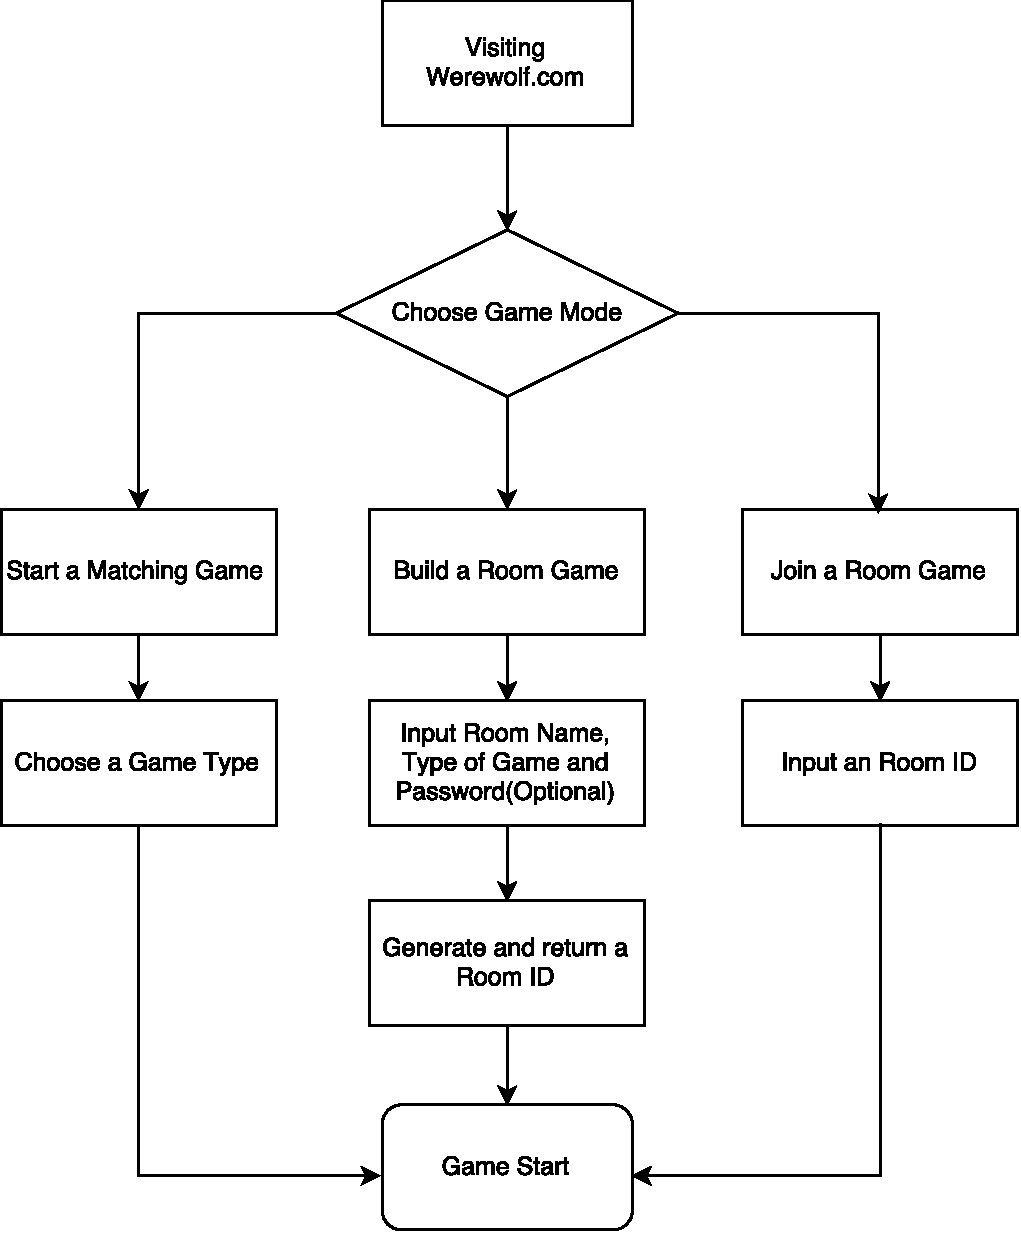
\includegraphics[width=0.7\linewidth, keepaspectratio]{func-index.pdf}
\caption{Functionality: Index}
\label{fig:func-index}
\end{figure}

\begin{figure}
\centering
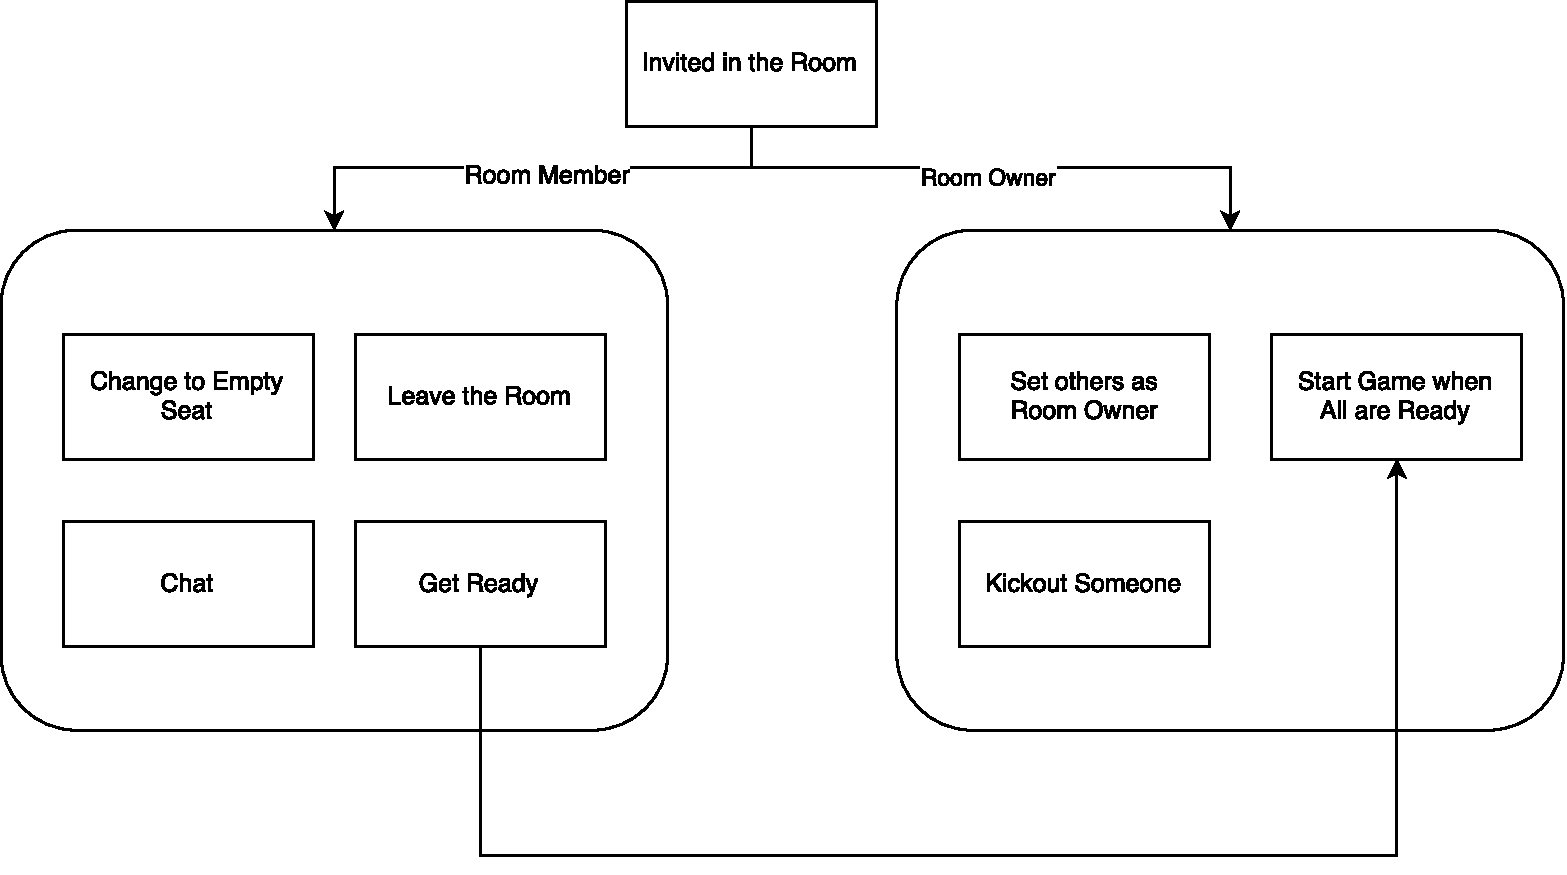
\includegraphics[width=0.7\linewidth, keepaspectratio]{func-inroom.pdf}
\caption{Functionality: In a Room}
\label{fig:func-inroom}
\end{figure}

\begin{figure}
\centering
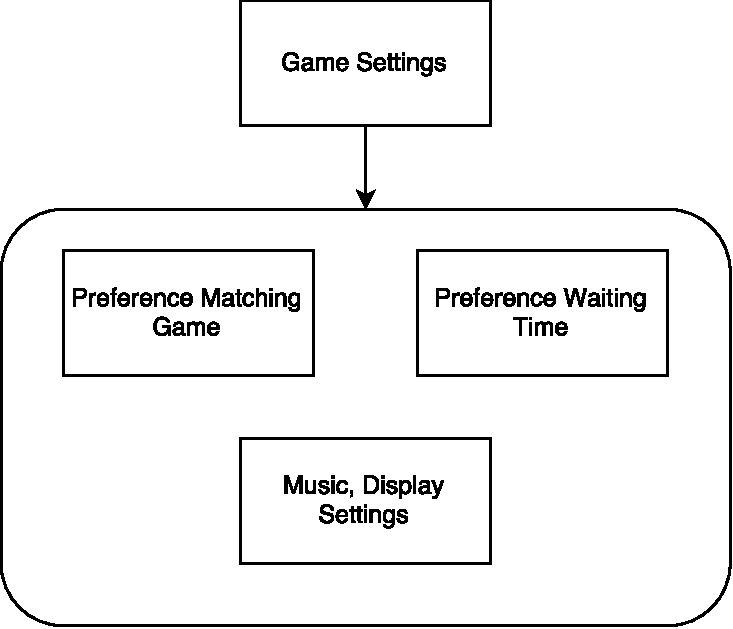
\includegraphics[width=0.7\linewidth, keepaspectratio]{func-settings.pdf}
\caption{Functionality: Game Settings}
\label{fig:func-settings}
\end{figure}

\begin{figure}
\centering
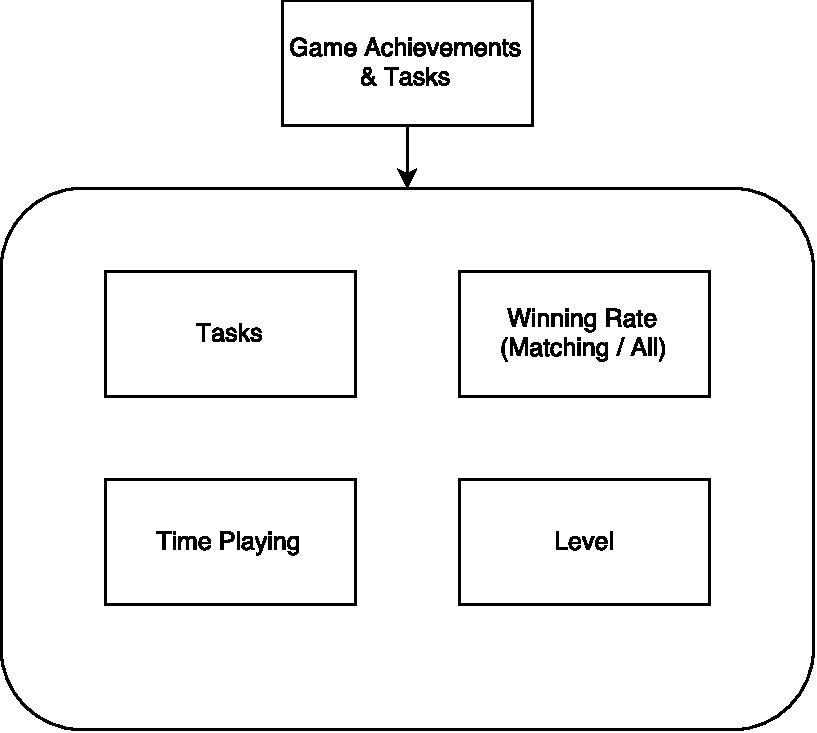
\includegraphics[width=0.7\linewidth, keepaspectratio]{func-tasks.pdf}
\caption{Functionality: Game Achievements \& Tasks}
\label{fig:func-tasks}
\end{figure}

\subsection{In a Game}

\begin{figure}
\centering
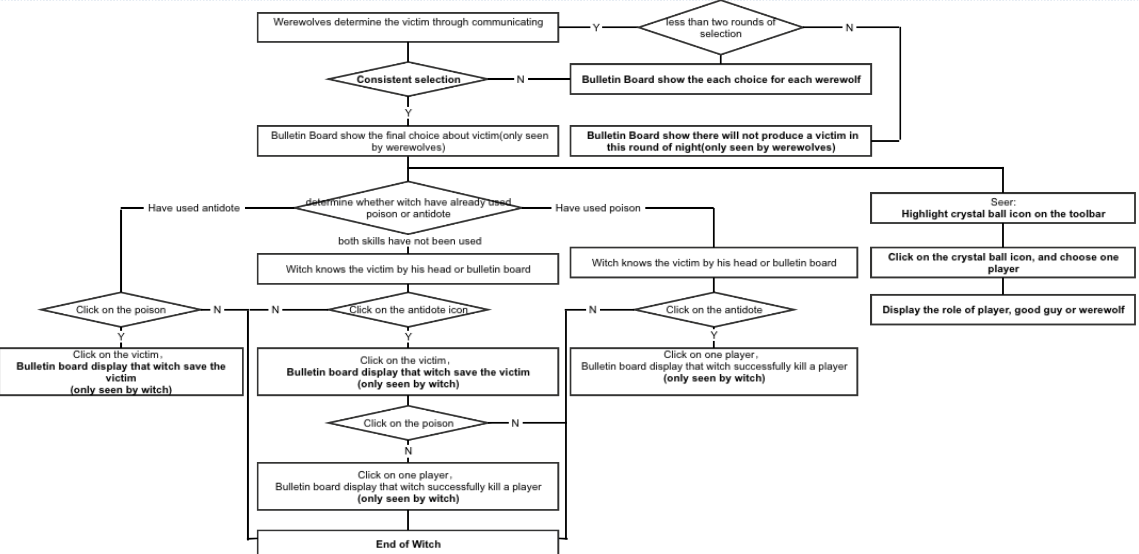
\includegraphics[width=0.7\linewidth, keepaspectratio]{func-gamenight.png}
\caption{Functionality: Game in the Night}
\label{fig:func-gamenight}
\end{figure}

\section{Data Model}

\section{Wireframes}

\begin{figure}
\centering
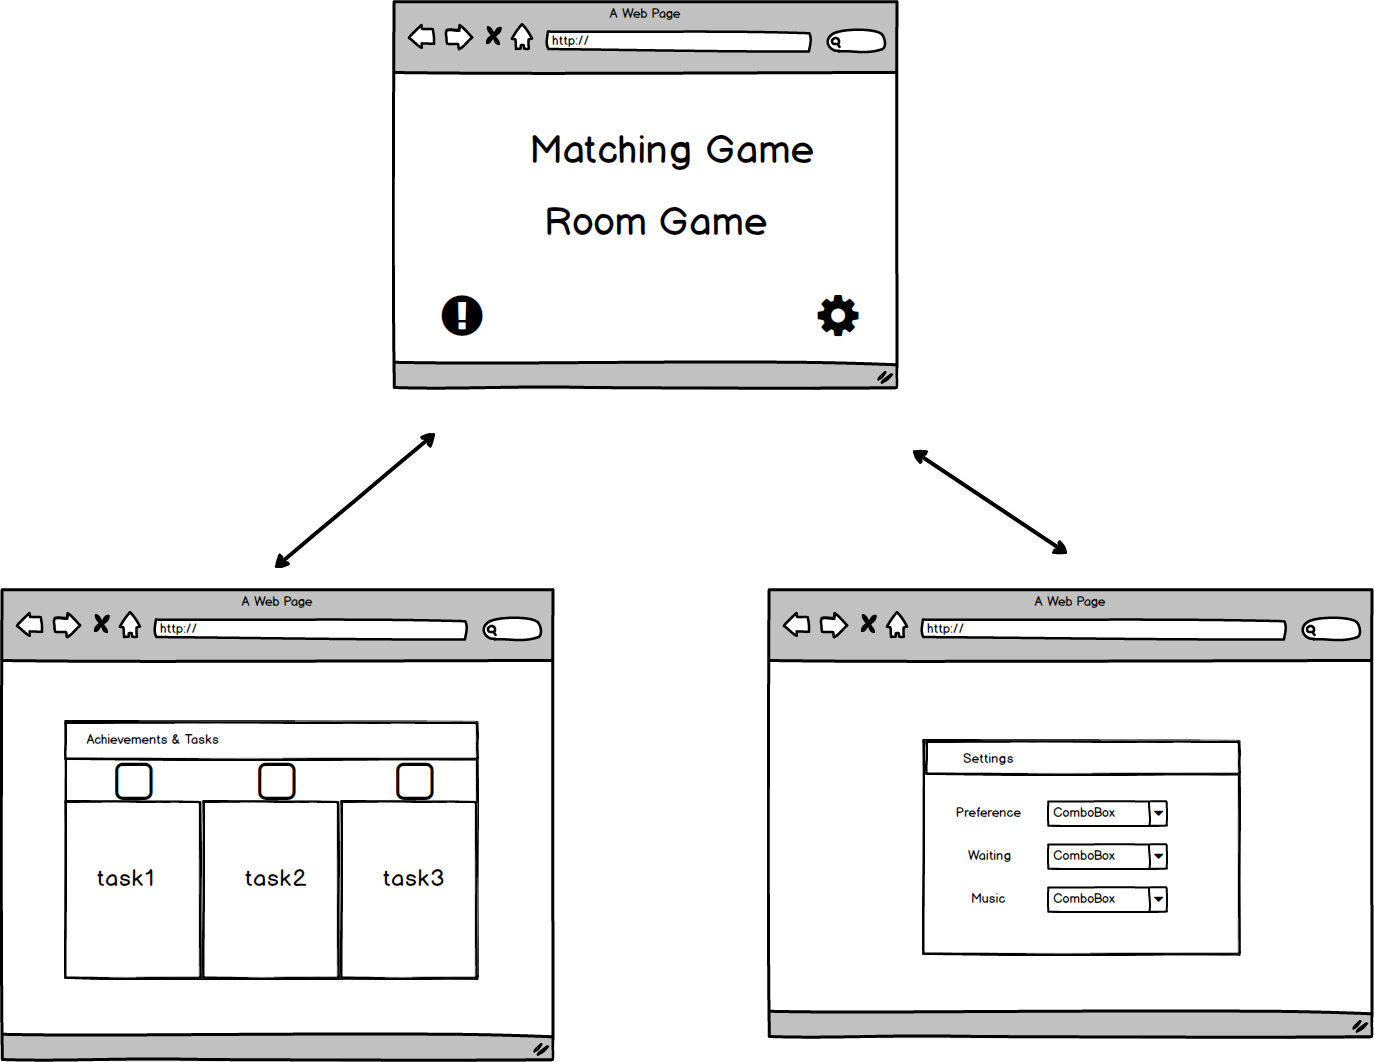
\includegraphics[width=0.7\linewidth, keepaspectratio]{wf-mainpage.png}
\caption{Wireframe: Main Page}
\label{fig:main}
\end{figure}

\begin{figure}
\centering
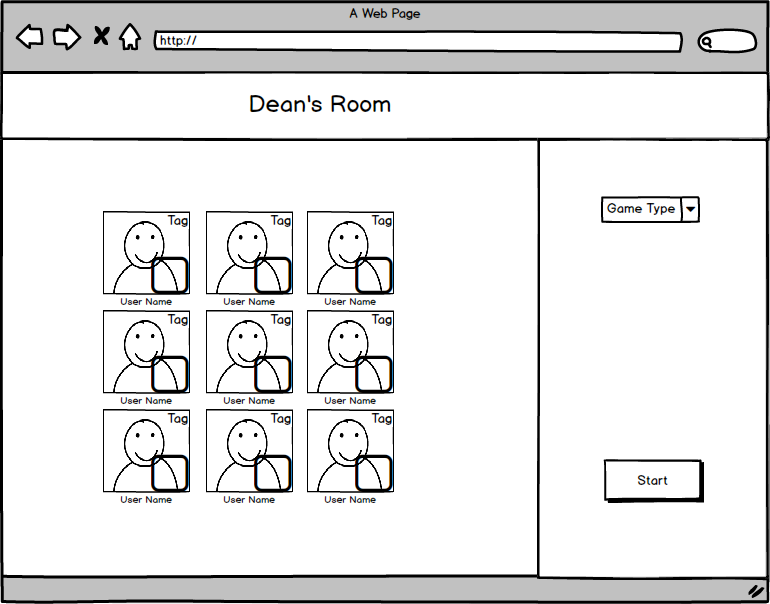
\includegraphics[width=0.7\linewidth, keepaspectratio]{wf-inroom.png}
\caption{Wireframe: Game Room}
\label{fig:room}
\end{figure}

\begin{figure}
\centering
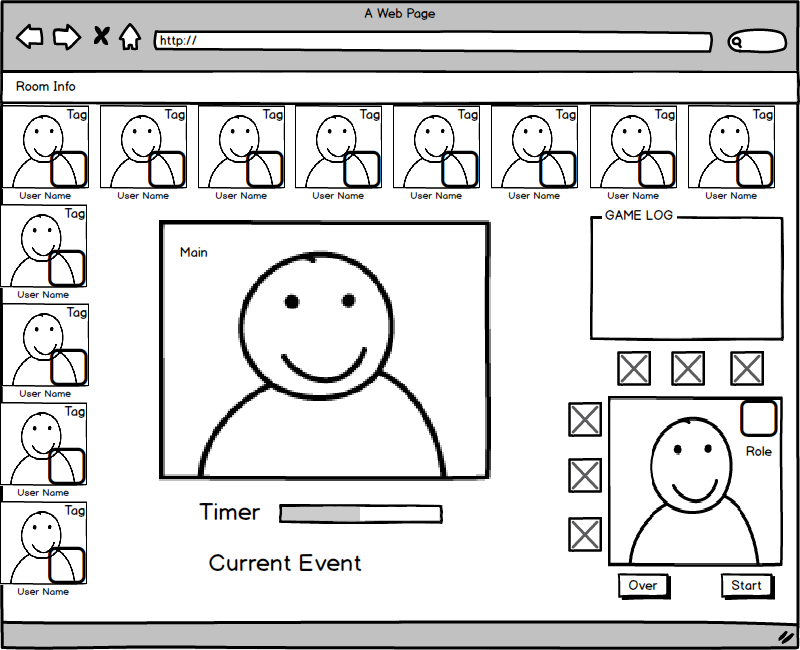
\includegraphics[width=0.7\linewidth, keepaspectratio]{wf-ingame.png}
\caption{Wireframe: Game View}
\label{fig:game}
\end{figure}

% For many users, the previous commands will be enough.
% If you want to directly input Unicode, add an Input Menu or Keyboard to the menu bar 
% using the International Panel in System Preferences.
% Unicode must be typeset using a font containing the appropriate characters.
% Remove the comment signs below for examples.

% \newfontfamily{\A}{Geeza Pro}
% \newfontfamily{\H}[Scale=0.9]{Lucida Grande}
% \newfontfamily{\J}[Scale=0.85]{Osaka}

% Here are some multilingual Unicode fonts: this is Arabic text: {\A السلام عليكم}, this is Hebrew: {\H שלום}, 
% and here's some Japanese: {\J 今日は}.



\end{document}  